\documentclass[11pt]{article}
\usepackage{microtype}
\usepackage{graphicx}
\usepackage{wrapfig}
\usepackage{url}
\usepackage{wrapfig}
\usepackage{color}
\usepackage{marvosym}
\usepackage{enumerate}
\usepackage{subfigure}
\usepackage{tikz}
\usepackage[fleqn]{amsmath}
\DeclareMathOperator*{\argmax}{arg\,max}
\DeclareMathOperator*{\argmin}{arg\,min}
\usepackage{amssymb}
\usepackage{hyperref}
\usepackage[many]{tcolorbox}
\usepackage{lipsum}
\usepackage{float}
\usepackage{trimclip}
\usepackage{listings}
\usepackage{environ}% http://ctan.org/pkg/environ
\usepackage{wasysym}
\usepackage{array}
\usepackage{graphicx}
\graphicspath{ {./} }

\def\ci{\perp\!\!\!\perp}

\oddsidemargin 0mm
\evensidemargin 5mm
\topmargin -20mm
\textheight 240mm
\textwidth 160mm

\newcommand{\vwi}{{\bf w}_i}
\newcommand{\vw}{{\bf w}}
\newcommand{\vx}{{\bf x}}
\newcommand{\vy}{{\bf y}}
\newcommand{\vxi}{{\bf x}_i}
\newcommand{\yi}{y_i}
\newcommand{\vxj}{{\bf x}_j}
\newcommand{\vxn}{{\bf x}_n}
\newcommand{\yj}{y_j}
\newcommand{\ai}{\alpha_i}
\newcommand{\aj}{\alpha_j}
\newcommand{\X}{{\bf X}}
\newcommand{\Y}{{\bf Y}}
\newcommand{\vz}{{\bf z}}
\newcommand{\msigma}{{\bf \Sigma}}
\newcommand{\vmu}{{\bf \mu}}
\newcommand{\vmuk}{{\bf \mu}_k}
\newcommand{\msigmak}{{\bf \Sigma}_k}
\newcommand{\vmuj}{{\bf \mu}_j}
\newcommand{\msigmaj}{{\bf \Sigma}_j}
\newcommand{\pij}{\pi_j}
\newcommand{\pik}{\pi_k}
\newcommand{\D}{\mathcal{D}}
\newcommand{\el}{\mathcal{L}}
\newcommand{\N}{\mathcal{N}}
\newcommand{\vxij}{{\bf x}_{ij}}
\newcommand{\vt}{{\bf t}}
\newcommand{\yh}{\hat{y}}
\newcommand{\code}[1]{{\footnotesize \tt #1}}
\newcommand{\alphai}{\alpha_i}
\newcommand{\defeq}{\overset{\text{def}}{=}}
\renewcommand{\vec}[1]{\mathbf{#1}}


\bgroup
\def\arraystretch{1.5}
\newcolumntype{x}[1]{>{\centering\arraybackslash\hspace{0pt}}p{#1}}
\newcolumntype{z}[1]{>{\centering\arraybackslash}m{#1}}

%Arguments are 1 - height, 2 - box title
\newtcolorbox{textanswerbox}[2]{%
 width=\textwidth,colback=white,colframe=blue!30!black,floatplacement=H,height=#1,title=#2,clip lower=true,before upper={\parindent0em}}

 \newtcolorbox{eqanswerbox}[1]{%
 width=#1,colback=white,colframe=black,floatplacement=H,height=3em,sharp corners=all,clip lower=true,before upper={\parindent0em}}

 %Arguments are 1 - height, 2 - box title
 \NewEnviron{answertext}[2]{
        \noindent
        \marginbox*{0pt 10pt}{
        \clipbox{0pt 0pt 0pt 0pt}{
        \begin{textanswerbox}{#1}{#2}
        \BODY
        \end{textanswerbox}
        }
        }
}

%Arguments are 1 - height, 2 - box title, 3 - column definition
 \NewEnviron{answertable}[3]{
        \noindent
        \marginbox*{0pt 10pt}{
        \clipbox{0pt 0pt 0pt 0pt}{
        \begin{textanswerbox}{#1}{#2}
                \vspace{-0.5cm}
                        \begin{table}[H]
                        \centering
                        \begin{tabular}{#3}
                                \BODY
                        \end{tabular}
                        \end{table}
        \end{textanswerbox}
        }
        }
}

 %Arguments are 1 - height, 2 - box title, 3 - title, 4- equation label, 5 - equation box width
 \NewEnviron{answerequation}[5]{
        \noindent
        \marginbox*{0pt 10pt}{
        \clipbox{0pt 0pt 0pt 0pt}{
        \begin{textanswerbox}{#1}{#2}
                \vspace{-0.5cm}
                        \begin{table}[H]
                        \centering
                \renewcommand{\arraystretch}{0.5}% Tighter

                        \begin{tabular}{#3}
                                #4 =	&
                        \clipbox{0pt 0pt 0pt 0pt}{

                        \begin{eqanswerbox}{#5}
                                $\BODY$
                        \end{eqanswerbox}
                        } \\
                        \end{tabular}
                        \end{table}

        \end{textanswerbox}
        }
        }
}

 %Arguments are 1 - height, 2 - box title
 \NewEnviron{answerderivation}[2]{
        \noindent
        \marginbox*{0pt 10pt}{
        \clipbox{0pt 0pt 0pt 0pt}{
        \begin{textanswerbox}{#1}{#2}
        \BODY
        \end{textanswerbox}
        }
        }
}

\newcommand{\Checked}{{\LARGE \XBox}}%
\newcommand{\Unchecked}{{\LARGE \Square}}%
\newcommand{\TextRequired}{{\textbf{Place Answer Here}}}%
\newcommand{\EquationRequired}{\textbf{Type Equation Here}}%

\usetikzlibrary{shapes, arrows, calc, positioning,matrix}
\tikzset{
data/.style={circle, draw, text centered, minimum height=3em ,minimum width = .5em, inner sep = 2pt},
empty/.style={circle, text centered, minimum height=3em ,minimum width = .5em, inner sep = 2pt},
}
\newcommand{\ztnodesize}{.6}
\newcommand{\factorsize}{1}
\newcommand{\nodesize}{1.3}

\newcommand{\answertextheight}{5cm}
\newcommand{\answertableheight}{4cm}
\newcommand{\answerequationheight}{2.5cm}
\newcommand{\answerderivationheight}{14cm}

\newcounter{QuestionCounter}
\newcounter{SubQuestionCounter}[QuestionCounter]
\setcounter{SubQuestionCounter}{1}

\newcommand{\subquestiontitle}{Question \theQuestionCounter.\theSubQuestionCounter~}
\newcommand{\newquestion}{\stepcounter{QuestionCounter}\setcounter{SubQuestionCounter}{1}\newpage}
\newcommand{\newsubquestion}{\stepcounter{SubQuestionCounter}}

\DeclareMathOperator{\rank}{rank}
\DeclareMathOperator{\indices}{indices}
\DeclareMathOperator{\Bernoulli}{Bernoulli}
\DeclareMathOperator{\Bin}{Bin}
\DeclareMathOperator{\E}{E}
\DeclareMathOperator{\Var}{Var}
\DeclareMathOperator{\Cov}{Cov}

\lstset{language=[LaTeX]TeX,basicstyle=\ttfamily\bf}

\pagestyle{myheadings}
\markboth{Homework 4}{Fall 2021 CS 475/675 Machine Learning: Homework 4}

\title{CS 475 Machine Learning: Homework 4 Analytical \\
(70 points)\\
\Large{Assigned: Monday, Nov. 1st, 2021} \\
\Large{Due: Monday, Nov. 15th, 2021, 11:59 pm US/Eastern}}
\author{Partner 1: Chang Yan (cyan13), Partner 2:  Jingguo Liang (jliang35)}
\date{}

\begin{document}
\maketitle
\thispagestyle{headings}

\section*{Instructions }
We have provided this \LaTeX{} document for turning in this homework. We give you one or more boxes to answer each question.  The question to answer for each box will be noted in the title of the box.  You can change the size of the box if you need more space.\\

{\bf Other than your name, do not type anything outside the boxes. Leave the rest of the document unchanged.}\\


\textbf{
%Do not change any formatting in this document, or we may be unable to
  %grade your work. This includes, but is not limited to, the height of
  %textboxes, font sizes, and the spacing of text and tables.  Additionally,
  Do
  not add text outside of the answer boxes.  You are allowed to make boxes larger if needed.
  % Entering your answers are the only
  %changes allowed.
  }\\


\textbf{We strongly recommend you review your answers in the generated PDF to
  ensure they appear correct. We will grade what appears in the answer boxes in
  the submitted PDF, NOT the original latex file.}

% -----------------------------------------------------------

\pagebreak
\section*{MRFs}

{\bf Question 1.}

Consider the graphical model shown in Figure 1. In this model, $\vx$ is a sequence of observations for which we want to output a prediction $\vy$, which itself is a sequence, where the size of $\vy$ is the same as $\vx$. Assume that the potential functions have a log-linear form: $\psi(Z) = \exp\{\sum_i \theta_i f_i(Z)\}$, where $Z$ is the set of nodes that are arguments to the potential function (i.e. some combination of nodes in $\vx$ and $\vy$,) $\theta$ are the parameters of the potential functions and $f_i$ is a feature function.

\begin{small}
\begin{figure}[h]
    \begin{center}
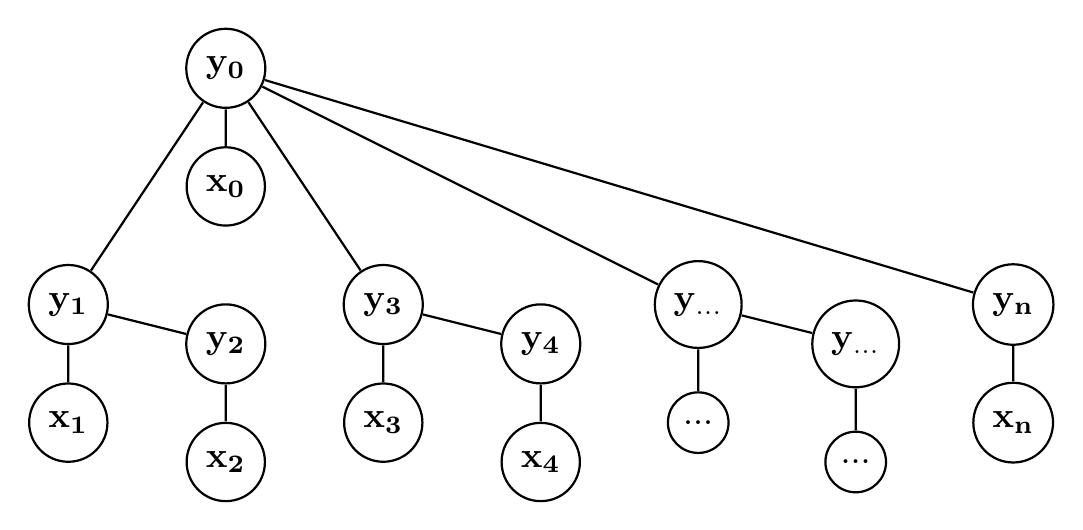
\begin{tikzpicture}[style=thick,scale=1]
            \begin{scope}[shape=circle,minimum size=0.1cm]
            \tikzstyle{every node}=[draw,fill]
            
            \node[fill=none,scale=\nodesize] (y_0) at (2,4.5) {$\mathbf{y_{0}}$};
            \node[fill=none,scale=\nodesize] (X_0) at (2,3) {$\mathbf{x_0}$};
            
            \node[fill=none,scale=\nodesize] (y_1) at (0,1.5) {$\mathbf{y_{1}}$};
            \node[fill=none,scale=\nodesize] (X_1) at (0,0) {$\mathbf{x_1}$};
            \node[fill=none,scale=\nodesize] (y_10) at (2,1.0) {$\mathbf{y_{2}}$};
            \node[fill=none,scale=\nodesize] (X_10) at (2,-0.5) {$\mathbf{x_2}$};
            
            \node[fill=none,scale=\nodesize] (y_2) at (4,1.5) {$\mathbf{y_{3}}$};
            \node[fill=none,scale=\nodesize] (X_2) at (4,0) {$\mathbf{x_3}$};
            \node[fill=none,scale=\nodesize] (y_20) at (6,1.0) {$\mathbf{y_{4}}$};
            \node[fill=none,scale=\nodesize] (X_20) at (6,-0.5) {$\mathbf{x_4}$};
            
            \node[fill=none,scale=\nodesize] (y_3) at (8,1.5) {$\mathbf{y_{\ldots}}$};
            \node[fill=none,scale=\nodesize] (X_3) at (8,0) {$\mathbf{...}$};
            \node[fill=none,scale=\nodesize] (y_30) at (10,1.0) {$\mathbf{y_{\ldots}}$};
            \node[fill=none,scale=\nodesize] (X_30) at (10,-0.5) {$\mathbf{...}$};          
            
            \node[fill=none,scale=\nodesize] (y_4) at (12,1.5) {$\mathbf{y_{n}}$};
            \node[fill=none,scale=\nodesize] (X_4) at (12,0) {$\mathbf{x_n}$};
            
            \draw [-] (X_0) -- (y_0);
            
            \draw [-] (y_0) -- (y_1);
            \draw [-] (X_1) -- (y_1);
            \draw [-] (y_1) -- (y_10);
            \draw [-] (X_10) -- (y_10);
            
            \draw [-] (y_0) -- (y_2);
            \draw [-] (X_2) -- (y_2);
            \draw [-] (y_2) -- (y_20);
            \draw [-] (X_20) -- (y_20);
            
            \draw [-] (y_0) -- (y_3);
            \draw [-] (X_3) -- (y_3);
            \draw [-] (y_3) -- (y_30);
            \draw [-] (X_30) -- (y_30);
            
            \draw [-] (y_0) -- (y_4);
            \draw [-] (X_4) -- (y_4);
            
            \end{scope}
        \end{tikzpicture}
            \caption{Tree structure model}
            \label{fig:tree_graph}
        \end{center}
\end{figure}
\end{small}

\begin{enumerate}
\item[(a)] Write the log likelihood for this model of a single instance $\vx$: $\log{p(\vy,\vx)}$. 

\item[(b)] Write the conditional log likelihood for this model of a single instance $\vx$: $\log{p(\vy|\vx)}$. 

\item[(c)] Assume that each variable $y_i$ can take one of $k$ possible states, and variable $x_i$ can take one of $k'$ possible states, where $k'$ is very large. Describe the computational challenges of modeling $\log p(\vy,\vx)$ vs $\log p(\vy|\vx)$.
\end{enumerate}

\begin{answertext}{15cm}{}

(a) \\
\begin{align*}
\log p(\vec{y}, \vec{x}) &= \log \left( \frac{1}{N} \prod_{\vec{Z}\in\mathcal{C}(\mathcal{G})} \psi_{\vec{Z}}(\vec{z}) \right) \\
&= \log \left( \frac{1}{N} \prod_{i=0}^{n} \psi(x_{i}, y_{i}) \prod_{j = 1,3,5,\ldots,n} \psi(y_{j}, y_{j+1}) \psi(y_{0}, y_{j}) \right) \\
&= \log \left( \frac{1}{N} \prod_{i=0}^{n} \exp( \theta_{x_{i}}f_{x_{i}}(x_{i}, y_{i}) + \theta_{y_{i}}f_{y_{i}}(x_{i}, y_{i})) \right.\\
	&\qquad \prod_{j = 1,3,5,\ldots,n} \exp( \theta_{y_{j}}f_{y_{j}}(y_{j}, y_{j+i}) + \theta_{y_{j+i}}f_{y_{j+i}}(y_{j}, y_{j+i})) \\
	&\qquad \left. \prod_{j = 1,3,5,\ldots,n} \exp( \theta_{y_{0}}f_{y_{j}}(y_{0}, y_{j}) + \theta_{y_{0}}f_{y_{j}}(y_{0}, y_{j}))  \right) \\
&= \log \left( \frac{1}{N} \right) \left[ \sum_{i=0}^{n} \left( \theta_{x_{i}}f_{x_{i}}(x_{i}, y_{i}) + \theta_{y_{i}}f_{y_{i}}(x_{i}, y_{i}) \right) \right. \\
	&\qquad + \sum_{j = 1,3,5,\ldots,n} \left( \theta_{y_{j}}f_{y_{j}}(y_{j}, y_{j+i}) + \theta_{y_{j+i}}f_{y_{j+i}}(y_{j}, y_{j+i}) \right) \\
	&\qquad \left. + \sum_{j = 1,3,5,\ldots,n} \left( \theta_{y_{0}}f_{y_{j}}(y_{0}, y_{j}) + \theta_{y_{0}}f_{y_{j}}(y_{0}, y_{j}) \right) \right]
\end{align*}

\end{answertext}

\newpage % for more space
\begin{answertext}{20cm}{}

(b)
\begin{align*}
\log p(\vec{y}\mid\vec{x}) &= \frac{\log p(\vec{y}, \vec{x})}{\sum_{y} \log p(\vec{y}, \vec{x})} \\
& = \log \left( \frac{1}{N} \right) \left[ \sum_{i=0}^{n} \left( \theta_{x_{i}}f_{x_{i}}(x_{i}, y_{i}) + \theta_{y_{i}}f_{y_{i}}(x_{i}, y_{i}) \right) \right. \\
	&\qquad + \sum_{j = 1,3,5,\ldots,n} \left( \theta_{y_{j}}f_{y_{j}}(y_{j}, y_{j+i}) + \theta_{y_{j+i}}f_{y_{j+i}}(y_{j}, y_{j+i}) \right) \\
	&\qquad \left. + \sum_{j = 1,3,5,\ldots,n} \left( \theta_{y_{0}}f_{y_{j}}(y_{0}, y_{j}) + \theta_{y_{0}}f_{y_{j}}(y_{0}, y_{j}) \right) \right] \\
	&\qquad \div \sum_{y} \log \left( \frac{1}{N} \right) \left[ \sum_{i=0}^{n} \left( \theta_{x_{i}}f_{x_{i}}(x_{i}, y_{i}) + \theta_{y_{i}}f_{y_{i}}(x_{i}, y_{i}) \right) \right. \\
	&\qquad + \sum_{j = 1,3,5,\ldots,n} \left( \theta_{y_{j}}f_{y_{j}}(y_{j}, y_{j+i}) + \theta_{y_{j+i}}f_{y_{j+i}}(y_{j}, y_{j+i}) \right) \\
	&\qquad \left. + \sum_{j = 1,3,5,\ldots,n} \left( \theta_{y_{0}}f_{y_{j}}(y_{0}, y_{j}) + \theta_{y_{0}}f_{y_{j}}(y_{0}, y_{j}) \right) \right]
\end{align*}

(c) \\
For $\log p(\vec{y}, \vec{x})$, we will have to evaluate approximately $2n$ $\psi(Z)$ functions, which is equivalent to $4n$ $f_{i}(Z)$ functions. And thus $4n$ additions are required to evaluate $\log p(\vec{y}, \vec{x})$. \\
For $\log p(\vec{y}\mid\vec{x})$, we have to evaluate $\log p(\vec{y}, \vec{x})$ for any possible enumeration of $\vec{y}$, which is $k^{n}$ possibilities. For each possible $\vec{y}$, the number of $f_{i}(Z)$ computation and additions is the same as above. Thus, a total of $4nk^{n}$ computation of $f_{i}(Z)$ function is required, as well as $4nk^{n}$ additions. We can see that the computational challenge here is much lager than that of $\log p(\vec{y}, \vec{x})$.\\

\end{answertext} 

\pagebreak
{\bf Question 2.}

\begin{enumerate}
\item[(a)] Suppose you wanted to compute $S = \sum^{100}_{x_1 = 1} \dots \sum^{100}_{x_8 = 1} h(x)$ where
\begin{equation*}
    h(x) = \exp(x_1 x_2 + x_4 x_5 + x_7 x_8) \prod_{i=2,5,7} (x_i + x_3 + x_6)^i.
\end{equation*}
It looks like the sum has $100^8 = 10^{16}$ terms, so it seems we must evaluate $h$ $10^{16}$ times. Explain (precisely) how you can compute $S$ with at most $10^7$ evaluations of $h$ or something simpler than $h$.

\item[(b)] Draw the MRF associated with this distribution.
\end{enumerate}

\begin{answertext}{24cm}{}
\begin{enumerate}
\item[(a)] The summation is:
\begin{align*}
S &= \sum^{100}_{x_1 = 1} \dots \sum^{100}_{x_8 = 1} \exp(x_1 x_2 + x_4 x_5 + x_7 x_8) \prod_{i=2,5,7} (x_i + x_3 + x_6)^i\\
&= \sum^{100}_{x_1 = 1} \dots \sum^{100}_{x_8 = 1} e^{x_1 x_2} e^{x_4 x_5} e^{x_7 x_8} \prod_{i=2,5,7} (x_i + x_3 + x_6)^i\\
&= \sum^{100}_{x_2 = 1} \dots \sum^{100}_{x_8 = 1} \left(\sum^{100}_{x_1 = 1} e^{x_1 x_2} \right) e^{x_4 x_5} e^{x_7 x_8} \prod_{i=2,5,7} (x_i + x_3 + x_6)^i
\end{align*}
Now we can compute the summation $\left(\sum^{100}_{x_1 = 1} e^{x_1 x_2} \right)$ easily as:
$$\phi^*_{x_2}(x_2) = \sum^{100}_{x_1 = 1} e^{x_1 x_2}$$
This is an object that is only a function of $x_2$. Thus, we can pre-evaluate it and store it as a mapping function (distribution) of $x_2$. Only need 100 spaces to store this mapping function, and as only two variables are involved, the computation of this mapping function would need to evaluate $e^{x_1 x_2}$ for $100^2=10^4$ times, so the total number of evaluations now is $10^4$\\
Then we can apply the same thing again to sum $x_4$:
$$S = \sum^{100}_{x_2 = 1} \sum^{100}_{x_3 = 1}\sum^{100}_{x_5 = 1}\dots\sum^{100}_{x_8 = 1}\phi^*_{x_2}(x_2) \left(\sum^{100}_{x_4 = 1} e^{x_4 x_5} \right) e^{x_7 x_8} \prod_{i=2,5,7} (x_i + x_3 + x_6)^i$$
Again we compute the summation $\left(\sum^{100}_{x_4 = 1} e^{x_4 x_5}\right)$ easily as a mapping function (distribution) of $x_5$:
$$\phi^*_{x_5}(x_5) = \sum^{100}_{x_4 = 1} e^{x_4 x_5}$$
We pre-evaluate this function and store it as a mapping function. Again, it requires 100 spaces and we need to evaluate $e^{x_4 x_5}$ for $100^2=10^4$ times, so the total number of evaluations now is $10^4 + 10^4=2\cdot 10^4$\\
We continue to apply this trick to sum $x_8$:
$$S = \sum^{100}_{x_2 = 1} \sum^{100}_{x_3 = 1}\sum^{100}_{x_5 = 1}\dots\sum^{100}_{x_7 = 1}\phi^*_{x_2}(x_2) \phi^*_{x_5}(x_5) \left(\sum^{100}_{x_8 = 1} e^{x_7 x_8}\right)  \prod_{i=2,5,7} (x_i + x_3 + x_6)^i$$
Compute summation $\left(\sum^{100}_{x_8 = 1} e^{x_7 x_8}\right)$ easily as mapping function (distribution) of $x_7$:
$$\phi^*_{x_7}(x_7) = \sum^{100}_{x_8 = 1} e^{x_7 x_8}$$
Again we pre-evaluate this function and store it as a mapping function, which requires 100 spaces and we need to evaluate $e^{x_7 x_8}$ for $100^2=10^4$ times, so the total number of evaluations now is $2\cdot10^4 + 10^4=3\cdot 10^4$\\
\end{enumerate}
\end{answertext} 
\begin{answertext}{24cm}{}
(Continued)\\
Now further expand our equation we have:
$$S = \sum^{100}_{x_2 = 1} \sum^{100}_{x_3 = 1}\sum^{100}_{x_5 = 1}\dots\sum^{100}_{x_7 = 1}\phi^*_{x_2}(x_2) \phi^*_{x_5}(x_5) \phi^*_{x_7}(x_7)  (x_2 + x_3 + x_6)^2 (x_5 + x_3 + x_6)^5 (x_7 + x_3 + x_6)^7$$
This time we can sum $x_2$ first:
$$S = \sum^{100}_{x_3 = 1}\sum^{100}_{x_5 = 1}\dots\sum^{100}_{x_7 = 1}\left(\sum^{100}_{x_2 = 1} \phi^*_{x_2}(x_2) (x_2 + x_3 + x_6)^2 \right) \phi^*_{x_5}(x_5) \phi^*_{x_7}(x_7)  \prod_{i=5,7} (x_i + x_3 + x_6)^i$$
We can compute the summation $\left(\sum^{100}_{x_2 = 1} \phi^*_{x_2}(x_2) (x_2 + x_3 + x_6)^2 \right)$ easily as mapping function (distribution) of $x_3$ and $x_6$:
$$\phi^{x_2\rightarrow}_{x_3,x_6}(x_3,x_6)= \sum^{100}_{x_2 = 1} \phi^*_{x_2}(x_2) (x_2 + x_3 + x_6)^2 $$
This is an object that is only a function of $x_3$ and $x_6$. Thus, we can pre-evaluate it and store it as a mapping function (distribution) of $x_3$ and $x_6$. This time we need $10^4$ spaces to store this mapping function, and as only three variables are involved, the computation of this mapping function would need to evaluate $\phi^*_{x_2}(x_2) (x_2 + x_3 + x_6)^2$ for $100^3=10^6$ times, so the total number of evaluations now is $3\cdot 10^4 + 10^6$\\
We apply the same trick to sum $x_5$:
$$S = \sum^{100}_{x_3 = 1}\sum^{100}_{x_6 = 1}\sum^{100}_{x_7 = 1}\phi^{x_2\rightarrow}_{x_3,x_6}(x_3,x_6)\left(\sum^{100}_{x_5 = 1} \phi^*_{x_5}(x_5) (x_5 + x_3 + x_6)^5 \right) \phi^*_{x_7}(x_7) (x_7 + x_3 + x_6)^7$$
Similarly we compute the summation $\left(\sum^{100}_{x_5 = 1} \phi^*_{x_5}(x_5) (x_5 + x_3 + x_6)^5 \right)$ as a mapping function (distribution) of $x_3$ and $x_6$:
$$\phi^{x_5\rightarrow}_{x_3,x_6}(x_3,x_6)= \sum^{100}_{x_5 = 1} \phi^*_{x_5}(x_5) (x_5 + x_3 + x_6)^5 $$
Again we pre-evaluate this function and store it as a mapping function, which requires $10^4$ spaces and we need to evaluate $\phi^*_{x_5}(x_5) (x_5 + x_3 + x_6)^5$ for $100^3=10^6$ times, so the total number of evaluations now is $3\cdot 10^4 + 10^6 + 10^6= 2\cdot 10^6 + 3\cdot 10^4$\\
Next we sum $x_7$
$$S = \sum^{100}_{x_3 = 1}\sum^{100}_{x_6 = 1}\phi^{x_2\rightarrow}_{x_3,x_6}(x_3,x_6) \phi^{x_5\rightarrow}_{x_3,x_6}(x_3,x_6) \left(\sum^{100}_{x_7 = 1} \phi^*_{x_7}(x_7) (x_7 + x_3 + x_6)^7 \right)$$
We compute summation $\left(\sum^{100}_{x_7 = 1} \phi^*_{x_7}(x_7) (x_7 + x_3 + x_6)^7 \right)$ easily as mapping function (distribution) of $x_3$ and $x_6$:
$$\phi^{x_7\rightarrow}_{x_3,x_6}(x_3,x_6)= \sum^{100}_{x_7 = 1} \phi^*_{x_7}(x_7) (x_7 + x_3 + x_6)^7 $$
next we sum $x_7$

\end{answertext} 
\begin{answertext}{20cm}{}
(Continued)
\begin{enumerate}
\item[]Once more we pre-evaluate this function and store it as a mapping function, which requires $10^4$ spaces and we need to evaluate $\phi^*_{x_7}(x_7) (x_7 + x_3 + x_6)^7$ for $100^3=10^6$ times, so the total number of evaluations now is $2\cdot 10^6 + 3\cdot 10^4 + 10^6= 3\cdot 10^6 + 3\cdot 10^4$\\
The final expression we need to evaluate looks like:
$$S = \sum^{100}_{x_3 = 1}\sum^{100}_{x_6 = 1}\phi^{x_2\rightarrow}_{x_3,x_6}(x_3,x_6) \phi^{x_5\rightarrow}_{x_3,x_6}(x_3,x_6) \phi^{x_7\rightarrow}_{x_3,x_6}(x_3,x_6)$$
All of $\phi^{x_2\rightarrow}_{x_3,x_6}(x_3,x_6) \ \text{,}\ \phi^{x_5\rightarrow}_{x_3,x_6}(x_3,x_6)\ \text{and} \ \phi^{x_7\rightarrow}_{x_3,x_6}(x_3,x_6)$ are mapping functions that we already computed and stored, so the evaluation of S now is fairly easy. We only need to sum over two variables $x_3$ and $x_6$, so the number of evaluation is $100^2 = 10^4$. The total time of evaluations now is: $3\cdot 10^6 + 3\cdot 10^4 + 10^4 = 3\cdot 10^6 + 4\cdot 10^4$. We can see clearly that:
$$3\cdot 10^6 + 4\cdot 10^4 < 10^7$$
So our total number of evaluations is less than $10^7$, and the method described above meets the requirement of this question.\\
\item[(b)] from part (a) we know from the equation and computation that we have 6 cliques in total: $(x_1, x_2),(x_4, x_5),(x_7, x_8),(x_3, x_6, x_2),(x_3, x_6, x_5),(x_3, x_6, x_7)$. We can draw a MRF that contains all of them:
\begin{center}
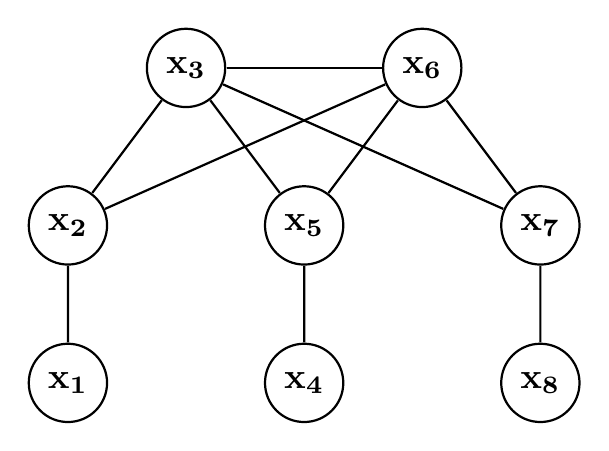
\begin{tikzpicture}[style=thick,scale=1]
            \begin{scope}[shape=circle,minimum size=0.1cm]
            \tikzstyle{every node}=[draw,fill]
            
            \node[fill=none,scale=\nodesize] (x_3) at (0,4) {$\mathbf{x_{3}}$};
            \node[fill=none,scale=\nodesize] (x_6) at (3,4) {$\mathbf{x_6}$};

            \node[fill=none,scale=\nodesize] (x_2) at (-1.5,2) {$\mathbf{x_{2}}$};
            \node[fill=none,scale=\nodesize] (x_5) at (1.5,2) {$\mathbf{x_5}$};
            \node[fill=none,scale=\nodesize] (x_7) at (4.5,2) {$\mathbf{x_{7}}$};   

            \node[fill=none,scale=\nodesize] (x_1) at (-1.5,0) {$\mathbf{x_{1}}$};
            \node[fill=none,scale=\nodesize] (x_4) at (1.5,0) {$\mathbf{x_4}$};
            \node[fill=none,scale=\nodesize] (x_8) at (4.5,0) {$\mathbf{x_{8}}$}; 

            
            \draw [-] (x_3) -- (x_6);

            \draw [-] (x_3) -- (x_2);
            \draw [-] (x_3) -- (x_5);
            \draw [-] (x_3) -- (x_7);

            \draw [-] (x_6) -- (x_2);
            \draw [-] (x_6) -- (x_5);
            \draw [-] (x_6) -- (x_7);

            \draw [-] (x_2) -- (x_1);
            \draw [-] (x_5) -- (x_4);
            \draw [-] (x_7) -- (x_8);
            
            \end{scope}
        \end{tikzpicture}
        \end{center}
\end{enumerate}
\end{answertext} 
\pagebreak

\section*{DAGs, Clique Trees and Message Passing.}

\begin{center}
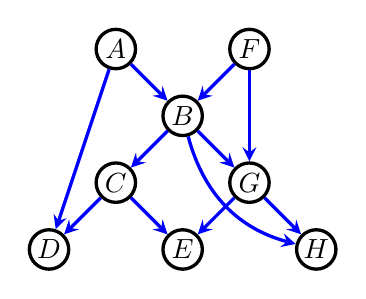
\begin{tikzpicture}[>=stealth, node distance=1.2cm]
    \tikzstyle{format} = [draw, very thick, circle, minimum size=5.0mm,
	inner sep=0pt]

	\begin{scope}
		\path[->, very thick]
			node[format] (A) {$A$}
			node[format, below right of=A] (B) {$B$}
			node[format, below left of=B] (C) {$C$}
			node[format, below left of=C] (D) {$D$}
			node[format, below right of=C] (E) {$E$}
			
			node[format, above right of=B] (F) {$F$}
			node[format, below right of=B] (G) {$G$}
			node[format, below right of=G] (H) {$H$}

			(A) edge[blue] (B)
			(B) edge[blue] (C)

			(C) edge[blue] (D)
			(C) edge[blue] (E)

			(F) edge[blue] (B)
			(B) edge[blue] (G)
			(G) edge[blue] (H)
			
			(A) edge[blue] (D)
			(B) edge[blue,bend right=30] (H)
			(F) edge[blue] (G)
			(G) edge[blue] (E)
		;
	\end{scope}
\end{tikzpicture}
\end{center}

In a statistical DAG model for the graph shown, let ${\bf V} = \{ A, B, C, D, E, F, G, H \}$.

\begin{itemize}
\item[(a)] Answer (and explain your answer) the following d-separation queries:
\begin{align*}
A &\ci F \mid D \\
A &\ci G \mid B,C\\
G &\ci A \mid  B,H,D,E,F\\
F &\ci D \mid A,B\\
C &\ci H \mid B
\end{align*}

\item[(b)] Write down the local Markov property of this model.

\item[(c)] Consider a new graph where we reverse the direction of the edge $B \to G$ to point the other way: $B \gets G$ (and leave the other edges the same).  Does the new graph represent the same model as the old?

Hint: write down the local Markov property for the new graph, and see if all statements in it are implied by d-separation in the original graph.  In general, if local Markov of ${\cal G}_1$ is implied by global Markov of ${\cal G}_2$, and local Markov of ${\cal G}_2$ is implied by global Markov of ${\cal G}_1$, then ${\cal G}_1$ and ${\cal G}_2$ represent the same model.  Otherwise they do not.

\item[(d)] A moralized graph ${\cal G}^a$ is obtained from a DAG ${\cal G}$ by connecting all non-adjacent variables $V_i$ and $V_j$ such
that $V_i \to V_k \gets V_j$ is in the graph (for some $V_k$), and replacing all directed edges by undirected edges.
What is the moralized graph for the DAG in this problem?

\item[(e)] Write down the MRF factorization of the moralized graph ${\cal G}^a$.

\item[(f)] Is this graph chordal?  If not, add a set of edges to make it chordal.  If you added edges, write the factorization of the new graph.

\item[(g)] Create a clique tree from the triangulated graph (either ${\cal G}^a$ or the graph obtained from ${\cal G}^a$ by adding new edge(s)).

\item[(h)] Pick a root $\vec{R}$ of the clique tree, and calculate both incoming messages $\phi^{\vec{S}_i\to\vec{S}_j}$ from each
$\vec{S}_i$ towards its neighbor $\vec{S}_j$ closer to the root, and outgoing messages $\phi^{\vec{S}_k\gets\vec{S}_i}$ from $\vec{S}_i$ to each neighbor $\vec{S}_k$ further than $\vec{S}_i$ from the root, in terms of clique potentials and other messages.

\item[(i)] By substituting in the clique factors in each message, show that in this example,

for each leaf node $\vec{S}_i$ with a neighbor node $\vec{S}_j$,
{\small
\begin{align*}
p(\vec{S}_i) =
\frac{
\phi^{\vec{S}_i \gets \vec{S}_j}_{\vec{S}_j \setminus \vec{S}_i} \phi_{\vec{S}_i}
}{
\sum_{\vec{S}_i}
\phi^{\vec{S}_i \gets \vec{S}_j}_{\vec{S}_j \setminus \vec{S}_i} \phi_{\vec{S}_i}
}
=
\frac{
\sum_{\vec{V} \setminus \vec{S}_i} \prod_{C \in {\cal C}({\cal G})} \phi_C
}{
\sum_{\vec{V}} \prod_{C \in {\cal C}({\cal G})} \phi_C
}
\end{align*}
}
for each non-leaf note $\vec{S}_i$ with a neighbor $\vec{S}_j$ closer to the root, and neighbors $\vec{S}_1, \ldots, \vec{S}_m$ further from the root that
{\small
\begin{align*}
p(\vec{S}_i) =
\frac{
\phi^{\vec{S}_i \gets \vec{S}_j}_{\vec{S}_j \setminus \vec{S}_i} 
\left( \prod_{k=1}^m \phi^{\vec{S}_k \to \vec{S}_i}_{\vec{S}_k \setminus \vec{S}_i} \right) \phi_{\vec{S}_i}
}{
\sum_{\vec{S}_i} \phi^{\vec{S}_i \gets \vec{S}_j}_{\vec{S}_j \setminus \vec{S}_i} 
\left( \prod_{k=1}^m \phi^{\vec{S}_k \to \vec{S}_i}_{\vec{S}_k \setminus \vec{S}_i} \right) \phi_{\vec{S}_i}
}
=
\frac{
\sum_{\vec{V} \setminus \vec{S}_i} \prod_{C \in {\cal C}({\cal G})} \phi_C
}{
\sum_{\vec{V}} \prod_{C \in {\cal C}({\cal G})} \phi_C
}
\end{align*}
}
and finally for the root node $\vec{S}_i$ with neighbors $\vec{S}_1, \ldots, \vec{S}_m$ that
{\small
\begin{align*}
p(\vec{S}_i) =
\frac{
\left( \prod_{k=1}^m \phi^{\vec{S}_k \to \vec{S}_i}_{\vec{S}_k \setminus \vec{S}_i} \right) \phi_{\vec{S}_i}
}{
\sum_{\vec{S}_i} \left( \prod_{k=1}^m \phi^{\vec{S}_k \to \vec{S}_i}_{\vec{S}_k \setminus \vec{S}_i} \right) \phi_{\vec{S}_i}
}
=
\frac{
\sum_{\vec{V} \setminus \vec{S}_i} \prod_{C \in {\cal C}({\cal G})} \phi_C
}{
\sum_{\vec{V}} \prod_{C \in {\cal C}({\cal G})} \phi_C
}
\end{align*}
}
\end{itemize}

Here $\vec{V}$ is all variables in the graph, and ${\cal C}({\cal G})$ is the set of maximal cliques in the graph.

\begin{answertext}{18cm}{}
\begin{itemize}

\item[(a)] Answer (and explain your answer) the following d-separation queries:
$$A \ci F \mid D $$
False. $A \rightarrow B \leftarrow F$ is a collider, and D is a descendant of B. Thus, when condition on D, A and F are not independent.
$$A \ci G \mid B,C$$
True. As we don't know D, $A \rightarrow D \leftarrow C$ is blocked. As we know B and C, $A \rightarrow B \rightarrow G$ and $B \rightarrow C \rightarrow G$ are blocked. As we don't know F and H, colliders $B \rightarrow F \leftarrow G$ and $B \rightarrow H \leftarrow G$ are also blocked. Thus, all paths from A to G are blocked, so A and G are independent.
$$G \ci A \mid  B,H,D,E,F$$
False. As we know D, collider $A \rightarrow D \leftarrow C$ is open. As we don't know C, split $D \leftarrow C \rightarrow E$ is open. Also we don't know E, so collider $C \rightarrow E \leftarrow G$ is open. Thus, path $A \rightarrow D \leftarrow C \rightarrow E \leftarrow G$ is open, and A and G are not independent.
$$F \ci D \mid A,B$$
True. As we know A, split $D \leftarrow A \rightarrow B$ is blocked. As we know B, directed $F \rightarrow B \rightarrow C$, $F \rightarrow B \rightarrow G$, and $F \rightarrow B \rightarrow H$ are blocked. Also, we don't know E, so the collider $C \rightarrow E \leftarrow G$ is blocked. Thus, all paths from F to D are blocked, so F and D are independent.
$$C \ci H \mid B$$
True. As we don't know E and D, colliders $A \rightarrow D \leftarrow C$ and $C \rightarrow E \leftarrow G$ are blocked. As we know B, split $C \leftarrow B \rightarrow G$ and $C \leftarrow B \rightarrow H$ are blocked, as well as directed $C \leftarrow B \leftarrow F$. Thus, all paths from C to H are blocked, so C and H are independent.

\end{itemize}
\end{answertext} 
\begin{answertext}{18cm}{}
\begin{itemize}
\item[(b)] The local Markov properties are:
\begin{align*}
A &\ci F \\
C &\ci A, F, G, H \mid B \\
D &\ci B, E, F, G, H \mid A, C \\
E &\ci A, B, D, F, H \mid C, G \\
F &\ci A \\
G &\ci A, C, D \mid B, F \\
H &\ci A, C, D, E, F \mid B, G
\end{align*}

\item[(c)]
The local Markov property for the new graph is
\begin{align*}
A &\ci F, G \\
C &\ci A, F, G, H \mid B \\
D &\ci B, E, F, G, H \mid A, C \\
E &\ci A, B, D, F, H \mid C, G \\
F &\ci A \\
G &\ci A \mid F \\
H &\ci A, C, D, E, F \mid B, G
\end{align*}

In the old graph when nothing is conditioned, using d-separation we know the triplet $A \rightarrow B \rightarrow G$ is an open path indicating that $A \not\ci G$. However, in the new graph the local Markov property indicates that $A \ci G$ given nothing. Thus, the new graph does not represent the same as the old. \\

\item[(d)] The moralized graph ${\cal G}^a$ is:\\
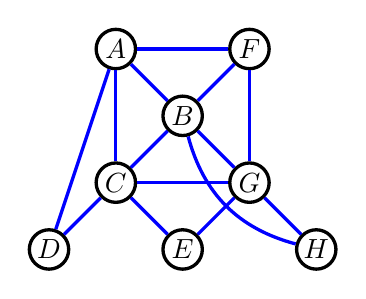
\begin{tikzpicture}[>=stealth, node distance=1.2cm]
    \tikzstyle{format} = [draw, very thick, circle, minimum size=5.0mm,
	inner sep=0pt]

	\begin{scope}
		\path[-, very thick]
			node[format] (A) {$A$}
			node[format, below right of=A] (B) {$B$}
			node[format, below left of=B] (C) {$C$}
			node[format, below left of=C] (D) {$D$}
			node[format, below right of=C] (E) {$E$}
			
			node[format, above right of=B] (F) {$F$}
			node[format, below right of=B] (G) {$G$}
			node[format, below right of=G] (H) {$H$}

			(A) edge[blue] (B)
			(B) edge[blue] (C)

			(C) edge[blue] (D)
			(C) edge[blue] (E)

			(F) edge[blue] (B)
			(B) edge[blue] (G)
			(G) edge[blue] (H)
			
			(A) edge[blue] (D)
			(B) edge[blue,bend right=30] (H)
			(F) edge[blue] (G)
			(G) edge[blue] (E)

                (A) edge[blue] (C) 
                (C) edge[blue] (G)
                (A) edge[blue] (F)
		;
	\end{scope}
\end{tikzpicture}
\end{itemize}
\end{answertext} 
\newpage

\begin{answertext}{24cm}{}

\begin{itemize}

\item[(e)] First we find all the maximum cliques:\\
 (A,D,C),(A,B,C),(A,B,F),(B,C,G),(B,G,F)(C,E,G),(B,G,H). \\The MRF factorization would be:
\begin{align*}
&p(A,B,C,D,E,F,G,H)\\
=&\frac{1}{Z}\phi_{A,D,C}(A,D,C)\phi_{A,B,C}(A,B,C)\phi_{A,B,F}(A,B,F)\phi_{B,C,G}(B,C,G)\\&\cdot\phi_{B,G,F}(B,G,F)\phi_{C,E,G}(C,E,G)\phi_{B,G,H}(B,G,H)
\end{align*}
\item[(f)] No, this is not chordal, as we have a cycle of size 4 (A-C-G-F-A) which does not have a edge not in the cycle connecting vertices in the cycle. Thus, we need to add a new edge to fix this. I add edge (A-G) to it. Now the graph looks like:
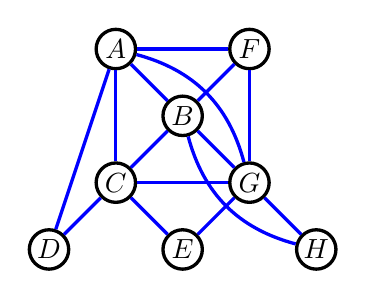
\begin{tikzpicture}[>=stealth, node distance=1.2cm]
    \tikzstyle{format} = [draw, very thick, circle, minimum size=5.0mm,
	inner sep=0pt]

	\begin{scope}
		\path[-, very thick]
			node[format] (A) {$A$}
			node[format, below right of=A] (B) {$B$}
			node[format, below left of=B] (C) {$C$}
			node[format, below left of=C] (D) {$D$}
			node[format, below right of=C] (E) {$E$}
			
			node[format, above right of=B] (F) {$F$}
			node[format, below right of=B] (G) {$G$}
			node[format, below right of=G] (H) {$H$}

			(A) edge[blue] (B)
			(B) edge[blue] (C)

			(C) edge[blue] (D)
			(C) edge[blue] (E)

			(F) edge[blue] (B)
			(B) edge[blue] (G)
			(G) edge[blue] (H)
			
			(A) edge[blue] (D)
			(B) edge[blue,bend right=30] (H)
			(F) edge[blue] (G)
			(G) edge[blue] (E)

                (A) edge[blue] (C) 
                (C) edge[blue] (G)
                (A) edge[blue] (F)
			(A) edge[blue,bend right=-30] (G)
		;
	\end{scope}
\end{tikzpicture}\\
Now the maximun cliques becomes:\\
(A,D,C),(A,B,C,G),(A,B,F,G),(C,E,G),(B,G,H).\\The MRF factorization would be:
\begin{align*}
&p(A,B,C,D,E,F,G,H)\\
=&\frac{1}{Z}\phi_{A,D,C}(A,D,C)\phi_{A,B,C,G}(A,B,C,G)\phi_{A,B,F,G}(A,B,F,G)\\&\cdot\phi_{C,E,G}(C,E,G)\phi_{B,G,H}(B,G,H)
\end{align*}
\item[(g)] The clique tree from the graph obtained from ${\cal G}^a$ by adding new edge(s) is:\\
First, the new vertices in clique tree are: $$V = {(A,D,C),(A,B,C,G),(A,B,F,G),(C,E,G),(B,G,H)}$$
Create tree with best order of V and draw edges with Running intersection property:
\begin{center}
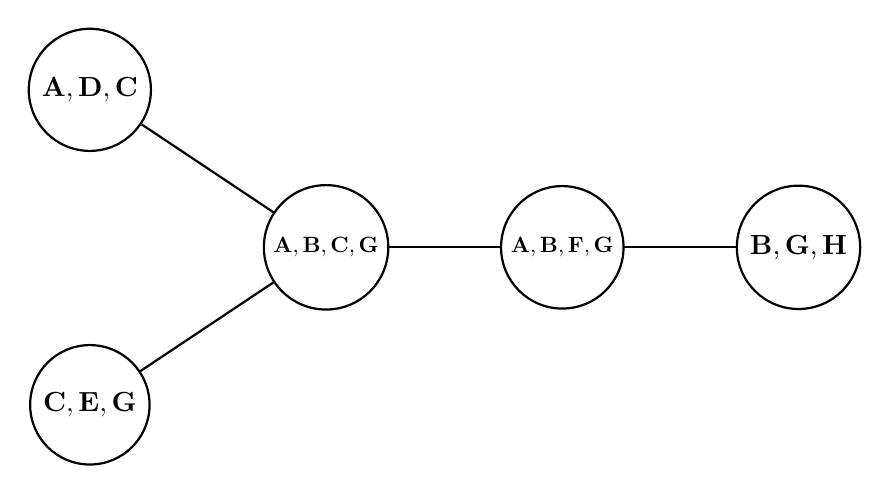
\begin{tikzpicture}[style=thick,scale=1]
            \begin{scope}[shape=circle,minimum size=0.1cm]
            \tikzstyle{every node}=[draw,fill]
            
            \node[fill=none,scale=1] (x_3) at (0,4) {$\mathbf{A,D,C}$};
            \node[fill=none,scale=1] (x_6) at (0,0) {$\mathbf{C,E,G}$};

            \node[fill=none,scale=0.8] (x_2) at (3,2) {$\mathbf{A,B,C,G}$};
            \node[fill=none,scale=0.8] (x_5) at (6,2) {$\mathbf{A,B,F,G}$};
            \node[fill=none,scale=1] (x_7) at (9,2) {$\mathbf{B,G,H}$};   
            
            \draw [-] (x_3) -- (x_2);

            \draw [-] (x_6) -- (x_2);
            \draw [-] (x_2) -- (x_5);
            \draw [-] (x_5) -- (x_7);
            
            \end{scope}
        \end{tikzpicture}
        \end{center}
\end{itemize}
To check the Running intersection property we can see the following graph: (next page)
\end{answertext} 
\begin{answertext}{23cm}{}

\begin{itemize}
\item[(g)] (Continued)\\
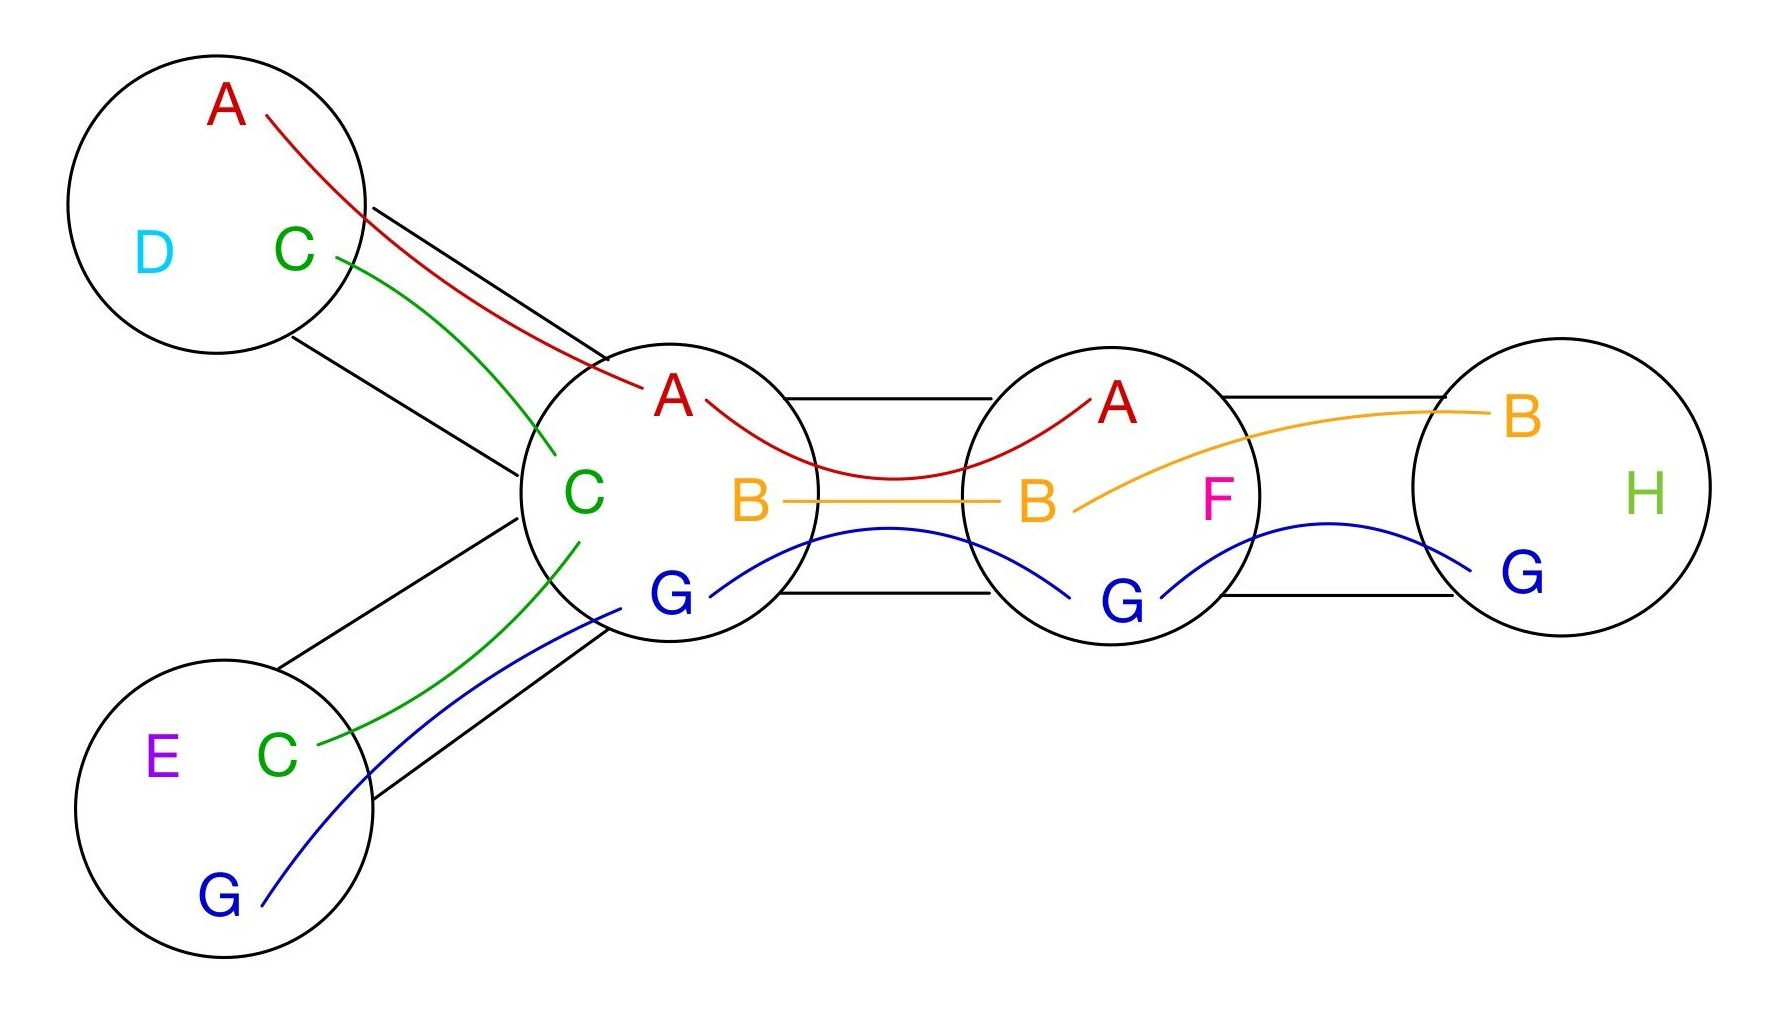
\includegraphics[scale=0.23]{tree}
\item[(h)] We name the nodes as $\vec{S}_{ADC},\vec{S}_{CEG},\vec{S}_{ABCG},\vec{S}_{ABFG}\text{ and }\vec{S}_{BGH}$ according to their original cliques, and choose vertex (B,G,H) ($\vec{S}_{BGH}$) as the Root $R$. The incoming messages are:

\begin{align*}
\phi^{\vec{S}_{ADC}\to\vec{S}_{ABCG}}&=\sum_{\vec{S}_{ADC}\backslash \vec{S}_{ABCG}}\phi_{\vec{S}_{ADC}}(\vec{S}_{ADC}) = \sum_{D}\phi_{\vec{S}_{ADC}}(\vec{S}_{ADC})\\
\phi^{\vec{S}_{CEG}\to\vec{S}_{ABCG}}&=\sum_{\vec{S}_{CEG}\backslash \vec{S}_{ABCG}}\phi_{\vec{S}_{CEG}}(\vec{S}_{CEG}) = \sum_{E}\phi_{\vec{S}_{CEG}}(\vec{S}_{CEG})
\end{align*}
\end{itemize}
\begin{align*}
\phi^{\vec{S}_{ABCG}\to\vec{S}_{ABFG}}&=\sum_{\vec{S}_{ABCG}\backslash \vec{S}_{ABFG}}\phi_{\vec{S}_{ABCG}}(\vec{S}_{ABCG})\prod_{\vec{S}_i=\vec{S}_{ADC},\vec{S}_{CEG}}\phi^{\vec{S}_i\to\vec{S}_{ABCG}}\\
&= \sum_{C}\phi_{\vec{S}_{ABCG}}(\vec{S}_{ABCG})\phi^{\vec{S}_{ADC}\to\vec{S}_{ABCG}}\phi^{\vec{S}_{CEG}\to\vec{S}_{ABCG}}\\
&= \sum_{C}\phi_{\vec{S}_{ABCG}}(\vec{S}_{ABCG})\sum_{D}\phi_{\vec{S}_{ADC}}(\vec{S}_{ADC})\sum_{E}\phi_{\vec{S}_{CEG}}(\vec{S}_{CEG})
\end{align*}
\begin{align*}
\phi^{\vec{S}_{ABFG}\to\vec{S}_{BGH}} &= \sum_{\vec{S}_{ABFG}\backslash\vec{S}_{BGH}} \phi_{\vec{S}_{ABFG}}(\vec{S}_{ABFG}) \,\phi^{\vec{S}_{ABCG}\to\vec{S}_{ABFG}} \\
&= \sum_{A,F} \phi_{\vec{S}_{ABFG}}(\vec{S}_{ABFG}) \,\sum_{C}\phi_{\vec{S}_{ABCG}}(\vec{S}_{ABCG})\\
&\qquad\sum_{D}\phi_{\vec{S}_{ADC}}(\vec{S}_{ADC})\sum_{E}\phi_{\vec{S}_{CEG}}(\vec{S}_{CEG})
\end{align*}

\end{answertext}

\begin{answertext}{23cm}{}
\begin{align*}
\phi^{\vec{S}_{ABFG}\leftarrow\vec{S}_{BGH}} &= \sum_{\vec{S}_{BGH}\backslash\vec{S}_{ABFG}} \phi_{\vec{S}_{BGH}}(\vec{S}_{BGH}) = \sum_{H} \phi_{\vec{S}_{BGH}}(\vec{S}_{BGH})
\end{align*}
\begin{align*}
\phi^{\vec{S}_{ABCG}\leftarrow\vec{S}_{ABFG}} &= \sum_{\vec{S}_{ABFG}\backslash\vec{S}_{ABCG}} \phi_{\vec{S}_{ABFG}}(\vec{S}_{ABFG}) \,\phi^{\vec{S}_{ABFG}\leftarrow\vec{S}_{BGH}} \\
&= \sum_{F} \phi_{\vec{S}_{ABFG}}(\vec{S}_{ABFG}) \sum_{H} \phi_{\vec{S}_{BGH}}(\vec{S}_{BGH})
\end{align*}
\begin{align*}
\phi^{\vec{S}_{ACD}\leftarrow\vec{S}_{ABCG}} &= \sum_{\vec{S}_{ABCG}\backslash\vec{S}_{ACD}} \phi_{\vec{S}_{ABCG}}(\vec{S}_{ABCG}) \,\phi^{\vec{S}_{ABCG}\leftarrow\vec{S}_{ABFG}} \,\phi^{\vec{S}_{CEG}\to\vec{S}_{ABCG}} \\
&= \sum_{B,G} \phi_{\vec{S}_{ABCG}}(\vec{S}_{ABCG}) \sum_{F} \phi_{\vec{S}_{ABFG}}(\vec{S}_{ABFG}) \sum_{H} \phi_{\vec{S}_{BGH}}(\vec{S}_{BGH}) \\
&\qquad\sum_{E}\phi_{\vec{S}_{CEG}}(\vec{S}_{CEG})
\end{align*}
\begin{align*}
\phi^{\vec{S}_{CEG}\leftarrow\vec{S}_{ABCG}} &= \sum_{\vec{S}_{ABCG}\backslash\vec{S}_{CEG}} \phi_{\vec{S}_{ABCG}}(\vec{S}_{ABCG}) \,\phi^{\vec{S}_{ABCG}\leftarrow\vec{S}_{ABFG}} \,\phi^{\vec{S}_{ACD}\to\vec{S}_{ABCG}} \\
&= \sum_{A,B} \phi_{\vec{S}_{ABCG}}(\vec{S}_{ABCG}) \sum_{F} \phi_{\vec{S}_{ABFG}}(\vec{S}_{ABFG}) \sum_{H} \phi_{\vec{S}_{BGH}}(\vec{S}_{BGH}) \\
&\qquad\sum_{D}\phi_{\vec{S}_{ADC}}(\vec{S}_{ADC})
\end{align*}
\end{answertext}
\pagebreak

% -----------------------------------------------------------

\section*{K-Means}

\begin{enumerate}
\item[(a)] Is it possible to initialize the k-means algorithm in such a way that it fails to terminate successfully?

\item[(b)] Say our input to k-means is a set of $2k$ points with 2-coordinates arranged in line, e.g. with coordinates:
{\small
\begin{align*}
(0,0), (0,1), (0, 2), \ldots, (0,k), (0,k+1), \ldots, (0,2k).
\end{align*}
}
Say we initialize $k$-means with 2 clusters, with initial centroids given by $(0,k)$ and $(0,k+1)$.  In many iterations will $k$-means terminate?  What will be the final cluster assignments and centroids?
\end{enumerate}

\begin{answertext}{18cm}{}
\begin{enumerate}
\item[(a)] No, it is not possible. By definition, k-means will always converge. In every iteration of k-means, the sum-of-distances to the center is reduced, and eventually it will stop changing, and the algorithm just terminate. Based on this definition, in each iteration the loss of k-mean will always decrease, or stay the same. The loss will never increase back, so the algorithm will always converge at some point of lower loss.\\


\item[(b)] It will terminate after just 2 iterations (the change only happens in the 1st iteration, and in the 2nd iteration nothing changes, so it terminates).\\
We can work out this step by step.\\ It is obvious that in the first step, (0,0),(0,1),...,(0,k) are closer to centroid (0, k), and (0,k+1),(0,k+2),...,(0,2k) are closer to centroid (0, k+1)
Thus, as x value is always 0, the new y value of the first centroid calculated from (0,0),(0,1)...(0,k) will be:
$$y_1 = \frac{0+1+2+...+k}{k+1}=\frac{(0+k)*(k+1)/2}{k+1}=\frac{(0+k)}{2}=\frac{k}{2}$$
Simiarly, the new value of y value of the second centroid calculated from (0,k+1),(0,k+2)...(0,2k) will be:
$$y_2 = \frac{(k+1) + (k+2) + ...+(2k)}{k}=\frac{(k+1+2k)*(k)/2}{k}=\frac{(3k+1)}{2}=\frac{3k}{2}+\frac{1}{2}$$
Now the new centroids are $(0,\frac{k}{2})$ and $(0,\frac{3k}{2}+\frac{1}{2})$.\\
Then in second iteration, it is obvious that most points will remain where the are, and we only need to check the edge cases (0,k) and (0,k+1). First we calculate the distance of (0,k) to both centroids:
$$d_1=|k-\frac{k}{2}|=\frac{k}{2}\ \ \ \ \ d_2=|\frac{3k}{2}+\frac{1}{2}-k|=\frac{k}{2}+\frac{1}{2}$$
We can see clearly that $d_1 < d_2$, so (0,k) is still closer to the first centroid and will remain in cluster 1.\\
Then we calculate the distance of (0,k+1) to both centroids:
$$d_1=|k+1-\frac{k}{2}|=\frac{k}{2}+1\ \ \ \ \ d_2=|\frac{3k}{2}+\frac{1}{2}-k-1|=\frac{k}{2}-\frac{1}{2}$$
We can see clearly that $d_1 > d_2$, so (0,k+1) is still closer to the second centroid and will remain in cluster 2.\\
\end{enumerate}
\end{answertext} 
\begin{answertext}{18cm}{}
(continued)\\
Thus, we can see that in iteration 2 nothing changes, so the algorithm will terminate. The number of iteration is 2 and the final cluster assignments and centroids are:\\
$$\text{Cluster 1: centroid: }\frac{k}{2}\text{ Points: }(0,0),(0,1),...,(0,k)$$
$$\text{Cluster 2: centroid: }\frac{3k}{2}+\frac{1}{2}\text{ Points: }(0,k+1),(0,k+2),...,(0,2k)$$
\end{answertext} 
\end{document}
